\section{随机变量的深入内容}

\subsection{随机变量的函数的分布}

\begin{theorem}[随机变量的函数]
设 $X$ 是离散随机变量,则 $Y=g(X)$ 的 PMF 为:
\[p_Y(y)=\sum_{\{x|y=g(x)\}}p_X(x)\]
设 $X$ 是连续随机变量,则 $Y=g(X)$ 的 CDF 为:
\[F_Y(y)=\Pb(Y\leqslant y)=\Pb(g(X)\leqslant y)=\int\limits_{\{x|g(x)\leqslant y\}}f_X(x)\mathrm dx\]
进而 PDF 为:
\[f_Y(y)=\frac{\mathrm d}{\mathrm dy}F_Y(y)\]
\end{theorem}

\begin{theorem}[线性函数情形]
\label{thm:rv-linear}
设 $X$ 是连续随机变量,$a,b\in\R$ 且 $a\neq0$,设 $Y=aX+b$,则:
\[f_Y(y)=\frac{1}{|a|}f_X\left(\frac{y-b}{a}\right)\]
\end{theorem}
\begin{proof}
先求 $Y$ 的 CDF:
\[F_Y(y)=\Pb(Y\leqslant y)=\Pb(aX+b\leqslant y)=\begin{cases}\Pb\left(X\leqslant \frac{y-b}{a}\right)=F_X\left(\frac{y-b}{a}\right),&a>0\\\Pb\left(X\geqslant \frac{y-b}{a}\right)=1-F_X\left(\frac{y-b}{a}\right),&a<0\end{cases}\]
然后求导得到 $Y$ 的 PDF:
\[f_Y(y)=\frac{\mathrm dF_Y(y)}{\mathrm dy}=\begin{cases}\frac{1}{a}f_X\left(\frac{y-b}{a}\right),&a>0\\-\frac{1}{a}f_X\left(\frac{y-b}{a}\right),&a<0\end{cases}\quad=\quad\frac{1}{|a|}f_X\left(\frac{y-b}{a}\right)\]
\end{proof}

\begin{example}[正态分布的线性变换仍然是正态分布]
设 $X\sim N(\mu,\sigma^2)$,$a,b\in\mathbb R$ 且 $a\neq0$,$Y=aX+b$,则根据定理 \ref{thm:rv-linear},有:
\begin{align*}
f_{Y}(y)&=\frac{1}{|a|}f_X\left(\frac{y-b}{a}\right)\\
&=\frac{1}{\sqrt{2\pi}\sigma|a|}\exp\left({-\frac{\left(\frac{y-b}{a}-\mu\right)^2}{2\sigma^2}}\right)\\
&=\frac{1}{\sqrt{2\pi}\sigma|a|}\exp\left({-\frac{(y-a\mu-b)^2}{2a^2\sigma^2}}\right)
\end{align*}
所以,$Y=aX+b\sim N(a\sigma+b,a^2\sigma^2)$.
\end{example}

\begin{theorem}[单调函数情形]
设 $X$ 是连续随机变量,$g$ 是严格单调的可逆函数,且其反函数 $h$ 可微,则 $Y=g(X)$ 在其支撑集 $\{y\mid f_Y(y)>0\}$ 上的 PDF 是:
\[f_Y(y)=f_X(h(y))\left|\frac{\mathrm d}{\mathrm dy}h(y)\right|\]
\end{theorem}
\begin{proof}
先求 $Y$ 的 CDF:
\[F_Y(y)=\Pb(Y\leqslant y)=\begin{cases}\Pb(X\leqslant h(y))=F_X(h(y)),&g\;\text{单调递增}\\\Pb(X\geqslant h(y))=1-F_X(h(y)),&g\;\text{单调递减}\end{cases}\]
于是求导得:
\[f_Y(y)=\begin{cases}f_X(h(y))h'(y),&g\;\text{单调递增}\\-f_X(h(y))h'(y),&g\;\text{单调递减}\end{cases}\quad =\quad f_X(h(y))\left|\frac{\mathrm d}{\mathrm dy}h(y)\right|\]
\end{proof}

\begin{theorem}[随机变量的二元函数]
设 $X,Y$ 是离散随机变量,则 $Z=g(X,Y)$ 的 PMF 为:
\[p_Z(z)=\sum_{\{(x,y)|z=g(x,y)\}}p_{X,Y}(x,y)\]
设 $X,Y$ 是连续随机变量,则 $Z=g(X,Y)$ 的 CDF 为:
\[F_Z(z)=\Pb(Z\leqslant z)=\Pb(g(X,Y)\leqslant z)=\iint\limits_{\{(x,y)|g(x,y)\leqslant z\}}f_{X,Y}(x,y)\mathrm dx\mathrm dy\]
进而 PDF 为:
\[f_Z(z)=\frac{\mathrm d}{\mathrm dz}F_Z(z)\]
\end{theorem}

\begin{example}[瑞利分布]
设 $X,Y\sim N(0,\sigma^2)$ 且相互独立,$R=\sqrt{X^2+Y^2}$,称 $R$ 服从瑞利分布。
首先计算 CDF:
\begin{align*}
F_R(r)&=\Pb(R\leqslant r)=\Pb(X^2+Y^2\leqslant r^2)\\
&=\iint\limits_{\{(x,y)|x^2+y^2\leqslant r^2\}}p_{X,Y}(x,y)\mathrm dx\mathrm dy\\
&=\iint\limits_{x^2+y^2\leqslant r^2}\frac{1}{2\pi\sigma^2}e^{-\frac{x^2+y^2}{2\sigma^2}}\mathrm dx\mathrm dy\\
&=\frac{1}{2\pi\sigma^2}\int_0^{2\pi}\mathrm d\theta\int_0^{r}e^{-\frac{\rho^2}{2\sigma^2}}\rho\mathrm d\rho\\
&=\left.e^{-\frac{\rho^2}{2\sigma^2}}\right|_{r}^0=1-e^{-\frac{r^2}{2\sigma^2}}
\end{align*}
故瑞利分布的 PDF 为:
\[f_R(r)=\frac{\mathrm dF_R(r)}{\mathrm dr}=\frac{r}{\sigma^2}e^{-\frac{r^2}{2\sigma^2}}\]
\end{example}

\begin{theorem}[极值分布]
设 $X,Y$ 是独立的随机变量,$M=\max(X,Y),N=\min(X,Y)$,则:
\[F_M(z)=F_X(z)F_Y(z),\qquad F_N(z)=1-(1-F_X(z))(1-F_Y(z))\]
\end{theorem}
\begin{proof}
\begin{align*}
F_M(z)&=\Pb(M\leqslant z)=\Pb(X\leqslant z, Y\leqslant z)=\Pb(X\leqslant z)\Pb(Y\leqslant z)=F_X(z)F_Y(z)\\
F_N(z)&=\Pb(N\leqslant z)=1-\Pb(N>z)=1-\Pb(X>z, Y>z)\\
&=1-\Pb(X>z)\Pb(Y>z)=1-(1-F_X(z))(1-F_Y(z))
\end{align*}
\end{proof}

\begin{corollary}
设 $X_1,X_2,\cdots,X_n$ 是 $n$ 个相互独立的随机变量,$M=\max\limits_{1\leqslant i\leqslant n}X_i$,$N=\min\limits_{1\leqslant i\leqslant n}X_i$,则:
\[F_M(z)=\prod_{i=1}^nF_{X_i}(z),\qquad F_N(z)=1-\prod_{i=1}^n(1-F_{X_i}(z))\]
\end{corollary}

\begin{theorem}[独立随机变量之和——卷积]
\label{thm:sum-ind-rv}
设 $X,Y$ 是独立的离散随机变量,$Z=X+Y$,则:
\[p_Z(z)=\sum_x p_X(x)p_Y(z-x)\]
设 $X,Y$ 是独立的连续随机变量,$Z=X+Y$,则:
\[f_Z(z)=\int_{-\infty}^{+\infty} f_X(x)f_Y(z-x)\mathrm dx\]
称上述两个式子为卷积(convolution)。
\end{theorem}

\begin{example}[独立正态随机变量之和仍服从正态分布]
设 $X\sim N(\mu_x,\sigma_x^2)$,$Y\sim N(\mu_y,\sigma_y^2)$ 且相互独立,$Z=X+Y$,则根据定理 \ref{thm:sum-ind-rv},有:
\[
f_Z(z)=\int_{-\infty}^{+\infty}\frac{1}{2\pi\sigma_x\sigma_y}e^{-\frac{(x-\mu_x)^2}{2\sigma_x^2}-\frac{(z-x-\mu_y)^2}{2\sigma_y^2}}\mathrm dx=\int_{-\infty}^{+\infty}\frac{1}{2\pi\sigma_x\sigma_y}e^{-\frac{1}{2}\left[\frac{u^2}{\sigma_x^2}+\frac{(v-u)^2}{\sigma_y^2}\right]}\mathrm du
\]
其中做了代换 $u=x-\mu_x,\,v=z-\mu_x-\mu_y$. 由于:
\[
\frac{u^2}{\sigma_x^2}+\frac{(v-u)^2}{\sigma_y^2}=\frac{u^2}{\sigma_x^2}+\frac{u^2}{\sigma_y^2}+\frac{v^2}{\sigma_y^2}-\frac{2uv}{\sigma_y^2}=\left(\frac{\sqrt{\sigma_x^2+\sigma_y^2}}{\sigma_x\sigma_y}u-\frac{\sigma_x v}{\sigma_y\sqrt{\sigma_x^2+\sigma_y^2}}\right)^2+\frac{v^2}{\sigma_x^2+\sigma_y^2}
\]
令 $t=\frac{\sqrt{\sigma_x^2+\sigma_y^2}}{\sigma_x\sigma_y}u-\frac{\sigma_x v}{\sigma_y\sqrt{\sigma_x^2+\sigma_y^2}}$,则:
\[
f_Z(z)=\frac{1}{2\pi\sigma_x\sigma_y}\frac{\sigma_x\sigma_y}{\sqrt{\sigma_x^2+\sigma_y^2}}e^{\frac{v^2}{\sigma_x^2+\sigma_y^2}}\int_{-\infty}^{+\infty}e^{-\frac{1}{2}t^2}\mathrm dt=\frac{1}{\sqrt{2\pi}\sqrt{\sigma_x^2+\sigma_y^2}}e^{\frac{(z-\mu_x-\mu_y)^2}{\sigma_x^2+\sigma_y^2}}
\]
所以 $Z\sim N(\mu_x+\mu_y,\sigma_x^2+\sigma_y^2)$.
\end{example}

\begin{example}[$n$ 个独立正态随机变量之和]
\label{ex:ind-normal-sum}
设 $X_i\sim N(\mu_i,\sigma_i^2),\,i=1,2,\ldots,n$ 且相互独立,则:
\[\sum\limits_{i=1}^nX_i\sim N\left(\sum\limits_{i=1}^n\mu_i,\sum\limits_{i=1}^n\sigma_i^2\right)\]
\end{example}

\begin{theorem}[随机变量的多元函数(可逆函数情形)]
设 $\mathbf{X}=(X_1,X_2,\cdots,X_n)$ 是一个随机向量,$T$ 是 $\R ^n$ 上的一可逆映射,$\mathbf Y=T(\mathbf X)$,则 $\mathbf Y$ 的 PDF 为:
\[f_{\mathbf Y}(\mathbf y)=f_{\mathbf X}(T^{-1}(\mathbf y))|J|\]
其中,$J$ 表示 $T^{-1}:\mathbf y\mapsto \mathbf x$,即 $\mathbf x=T^{-1}(\mathbf y)$ 的雅各比行列式:
\[
J=\begin{vmatrix}
\frac{\partial x_1}{\partial y_1}&\frac{\partial x_1}{\partial y_2}&\cdots&\frac{\partial x_1}{\partial y_n}\\
\frac{\partial x_2}{\partial y_1}&\frac{\partial x_2}{\partial y_2}&\cdots&\frac{\partial x_2}{\partial y_n}\\
\vdots&\vdots&\vdots&\vdots\\
\frac{\partial x_n}{\partial y_1}&\frac{\partial x_n}{\partial y_2}&\cdots&\frac{\partial x_n}{\partial y_n}\end{vmatrix}
\]
\end{theorem}
\begin{proof}
设 $D\subset \R^n$ 是一个性质好的集合,则:
\begin{align*}
\Pb(\mathbf Y\in D)&=\Pb(T(\mathbf X)\in D)\\
&=\Pb(\mathbf X\in T^{-1}(D))&\text{两边同时施以}\;T^{-1}\\
&=\int_{T^{-1}(D)}f_{\mathbf X}(\mathbf x)\mathrm d\mathbf x\\
&=\int_{D}f_{\mathbf X}(T^{-1}(y))|J|\mathrm d\mathbf y&\text{变量代换}\;\mathbf y=T(\mathbf x)
\end{align*}
又:
\[\Pb(\mathbf Y\in D)=\int_Df_\mathbf Y(\mathbf y)\mathrm d\mathbf y\]
根据 $D$ 一定的任意性,可知:
\[f_{\mathbf Y}(\mathbf y)=f_{\mathbf X}(T^{-1}(\mathbf y))|J|\]
\end{proof}


\subsection{协方差与相关系数}

\begin{figure}[H]
    \centering
    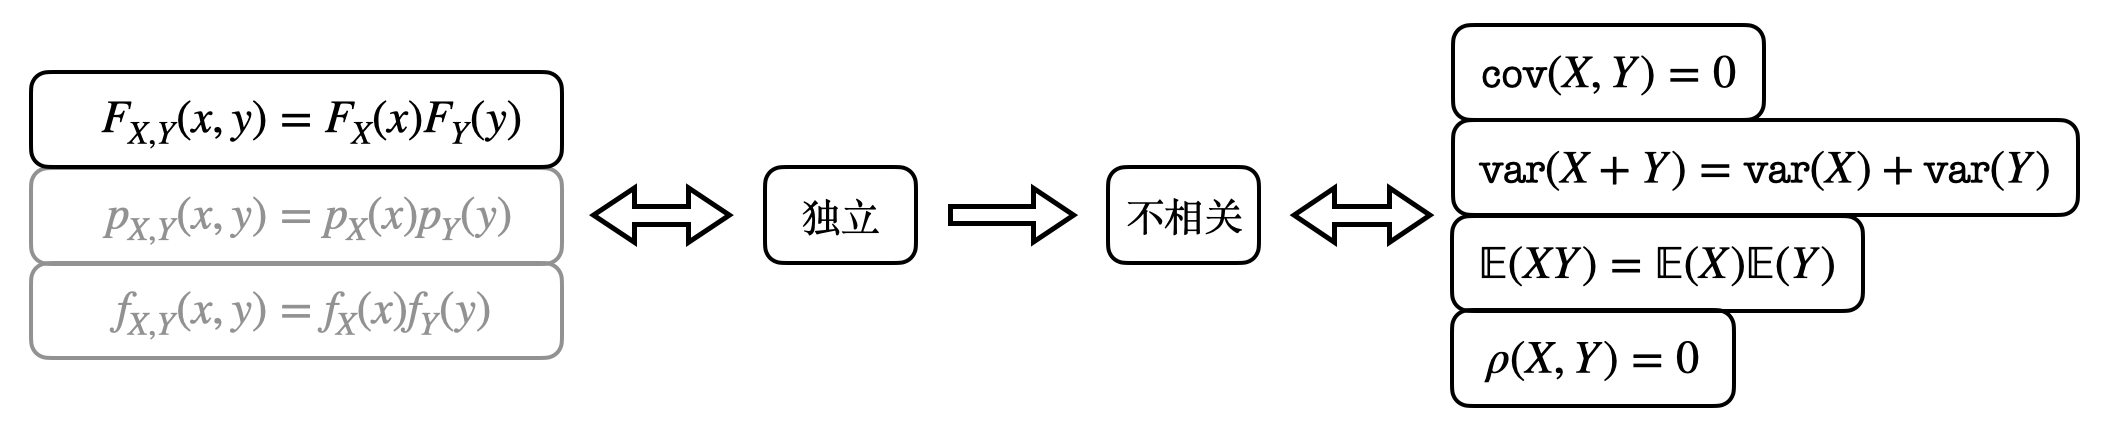
\includegraphics[width=0.9\linewidth]{figs/随机变量的独立性与相关性.png}
    \caption{随机变量的独立性与相关性示意图}
    \label{fig:independence-correlation}
\end{figure}

\begin{definition}[协方差与相关系数]
设 $X,Y$ 是两个随机变量,定义协方差与相关系数分别为:
\[
\cov(X,Y)=\E [(X-\E  X)(Y-\E  Y)],\quad\rho(X,Y)=\frac{\cov(X,Y)}{\sqrt{\var X\var Y}}
\]
当 $\cov(X,Y)=\rho(X,Y)=0$ 时,称 $X$ 和 $Y$ 不相关。
\end{definition}

\begin{property}
从定义出发容易证明以下性质:
\begin{itemize}
    \item $\cov(X,X)=\var(X)$
    \item $\cov(X,aY+b)=a\cdot\cov(X,Y)$ 
    \item $\cov(X,Y+Z)=\cov(X,Y)+\cov(X,Z)$
\end{itemize}
\end{property}

\begin{property}
$|\rho(X,Y)|\leq 1$.
\end{property}
\begin{proof}
对 $\forall t\in \R$,由于 $\var(Y-tX)=t^2\var X-2t\cov(X,Y)+\var Y\geq 0$,所以:
\[\Delta=4\cov^2(X,Y)-4\var X\var Y\leq 0\]
即有 $|\rho(X,Y)|\leq 1$.
\end{proof}

\begin{theorem}
设 $X,Y$ 是两个随机变量,则:
\[\cov(X,Y)=\E[XY]-\E X\E Y\]
\end{theorem}
\begin{proof}
\begin{align*}
\cov(X,Y)&=\E[(X-\E X)(Y-\E Y)]\\
&=\E[XY-\E X\cdot Y-X\cdot \E Y+\E X\E Y]\\
&=\E[XY]-\E X\cdot\E Y-\E X\cdot\E Y+\E X\cdot\E Y\\
&=\E[XY]-\E X\E Y
\end{align*}
\end{proof}

\begin{corollary}[独立与相关]
设 $X,Y$ 是两个随机变量,若 $X,Y$ 独立,则 $X,Y$ 不相关。
\end{corollary}
\begin{note}
反之不成立,不相关不能推出独立。
\end{note}

\begin{example}[不相关且不独立]
设随机变量 $X,Y$ 以 $1/4$ 的概率取 $(1,0),(0,1),(-1,0),(0,-1)$,则 $\E X=\E Y=\E[XY]=0$,于是 $\cov(X,Y)=\E[XY]-\E X\E Y=0$,故 $X,Y$ 不相关。但是 $p_{X,Y}(1,0)=1/4\neq p_X(1)p_Y(0)=1/4\cdot 1/2=1/8$,故二者不独立。直观上,$X$ 取非零值就要求 $Y$ 取零值,因此不独立。
\end{example}

\begin{theorem}[随机变量和的方差]
设随机变量 $X,Y$ 有有限的方差,则:
\[\var(X+Y)=\var X+2\cov(X,Y)+\var Y\]
更一般的,设随机变量 $X_1,X_2,\ldots,X_n$ 有有限的方差,则:
\[
\var\left(\sum_{i=1}^n X_i\right)=\sum_{i=1}^n\var(X_i)+\sum_{\{(i,j)\mid i\neq j\}}\cov(X_i,X_j)
\]
\end{theorem}
\begin{proof}
设 $\tilde X_i=X_i-\E[X_i]$,则:
\begin{align*}
\var\left(\sum_{i=1}^n X_i\right)&=\E\left[\left(\sum_{i=1}^n{\tilde X_i}^2\right)^2\right]\\
&=\E\left[\sum_{i=1}^n\sum_{j=1}^n\tilde X_i\tilde X_j\right]\\
&=\sum_{i=1}^n\sum_{j=1}^n\E\left[\tilde X_i\tilde X_j\right]\\
&=\sum_{i=1}^n\E[{\tilde X_i}^2]+\sum_{\{(i,j)\mid i\neq j\}}^n\E\left[\tilde X_i\tilde X_j\right]\\
&=\sum_{i=1}^n\var(X_i)+\sum_{\{(i,j)\mid i\neq j\}}\cov(X_i,X_j)
\end{align*}
\end{proof}

\begin{corollary}
设随机变量 $X,Y$ 有有限的方差,$a,b$ 为常数,则:
\[
\var(aX+bY)=a^2\var X+2ab\cov(X,Y)+b^2\var Y
\]
或写作矩阵形式:
\[
\var(aX+bY)=\begin{bmatrix}a&b\end{bmatrix}\begin{bmatrix}\var X&\cov(X,Y)\\\cov(Y,X)&\var Y\end{bmatrix}\begin{bmatrix}a\\b\end{bmatrix}
\]
\end{corollary}

% \begin{property}
% $\var(X)=0\implies \mathbb P(X=\E  X)=1$
% \end{property}
% \begin{proof}
% 根据切比雪夫不等式(见后文),$\mathbb P\left(|X-\E  X|\geq \frac{1}{n}\right)\leq n^2\var(X)=0$ 对 $\forall n$ 都成立,故 $\mathbb P(X=\E  X)=1$.
% \end{proof}

\subsection{再论条件期望与条件方差}
\label{sec:cond-e-cond-var}

\begin{definition}[条件期望作为估计量]
设 $X,Y$ 是随机变量,若将 $Y$ 视作能提供关于 $X$ 的信息的观测值,则可将条件期望视为给定 $Y$ 下对 $X$ 的估计,记作:
\[
\hat X=\E[X\vert Y]
\]
注意 $\hat X$ 是随机变量 $Y$ 的函数。进一步地,记估计误差为:
\[
\tilde X=\hat X-X
\]
则 $\tilde X$ 是随机变量 $X,Y$ 的二元函数。
\end{definition}

\begin{property}
根据全期望公式易知,条件期望是无偏估计,即 $\E\hat X=\E X$,或 $\E\tilde X=0$.
\end{property}

\begin{property}
$\E[\tilde X\vert Y]=0$,即对任意 $y$,都有 $\E[\tilde X\vert Y=y]=0$.
\end{property}
\begin{proof}
\[
\E[\tilde X\vert Y]=\E[(\hat X-X)\vert Y]=\E[\hat X\vert Y]-\E[X\vert Y]=\hat X-\hat X=0
\]
\end{proof}

\begin{property}
估计量 $\hat X$ 与估计误差 $\tilde X$ 不相关。
\end{property}
\begin{proof}
\[
\E[\hat X\tilde X]=\E[\E[\hat X\tilde X\vert Y]]=\E[\hat X\E[\tilde X\vert Y]]=0=\E\hat X\E\tilde X
\]
\end{proof}

\begin{property}
$\var(X)=\var(\hat X)+\var(\tilde X)$.
\end{property}
\begin{proof}
由于 $\hat X$ 与 $\tilde X$ 不相关,故 $\cov(\hat X,\tilde X)=0$,又 $X=\hat X+\tilde X$,故:
\[
\var(X)=\var(\hat X)+2\cov(\hat X,\tilde X)+\var(\tilde X)=\var(\hat X)+\var(\tilde X)
\]
\end{proof}


\subsection{矩母函数}

\begin{definition}[矩母函数]
设 $X$ 是一个随机变量,定义其矩母函数为:
\[
M_X(s)=\E[e^{sX}]=\begin{dcases}
    \sum_x e^{sx}p_X(x),&\text{$X$ 离散}\\
    \int_{-\infty}^{\infty} e^{sx}f_X(x)\mathrm dx,&\text{$X$ 连续}
\end{dcases}
\]
其定义域为使得 $\E[e^{sX}]$ 存在的 $s$. 在上下文清晰时可简记作 $M(s)$.
\end{definition}

\begin{theorem}[矩母函数计算矩]
设随机变量 $X$ 的矩母函数为 $M(s)$,则:
\[
\left.\frac{\mathrm d^n}{\mathrm ds^n}M(s)\right|_{s=0}=\E[X^n]
\]
\end{theorem}
\begin{proof}
假设积分(期望)与微分可交换,则:
\[
\frac{\mathrm d^n}{\mathrm ds^n}M(s)=\frac{\mathrm d^n}{\mathrm ds^n}\E[e^{sX}]=\E\left[\frac{\mathrm d^n}{\mathrm ds^n}e^{sX}\right]=\E[X^ne^{sX}]
\]
代入 $s=0$ 得:
\[
\left.\frac{\mathrm d^n}{\mathrm ds^n}M(s)\right|_{s=0}=\E[X^n]
\]
\end{proof}

\begin{theorem}[矩母函数与分布]
若随机变量 $X$ 的矩母函数 $M_X(s)$ 满足:存在一个正数 $a$,使得对 $\forall s\in[-a,a]$,$M_X(s)$ 都是有限的,则矩母函数 $M_X(s)$ 唯一决定 $X$ 的分布函数。
\end{theorem}

\begin{theorem}[独立随机变量之和]
设 $X,Y$ 是独立随机变量,$Z=X+Y$,则:
\[M_Z(s)=M_X(s)M_Y(s)\]
\end{theorem}
\begin{proof}
\[
M_Z(s)=\E[e^{sZ}]=\E[e^{s(X+Y)}]=\E[e^{sX}e^{sY}]=\E[e^{sX}]\E[e^{sY}]=M_X(s)M_Y(s)
\]
\end{proof}
\begin{corollary}
设 $X_1,X_2,\ldots,X_n$ 是独立随机变量,$Z=X_1+X_2+\cdots+X_n$,则:
\[
M_Z(s)=M_{X_1}(s)M_{X_2}(s)\cdots M_{X_n}(s)
\]
\end{corollary}

\begin{definition}[多元矩母函数]
设 $X_1,X_2,\ldots,X_n$ 是随机变量,定义它们的多元矩母函数为:
\[
M_{X_1,X_2,\ldots,X_n}(s_1,s_2,\ldots,s_n)=\E[e^{s_1X_1+s_2X_2+\cdots+s_nX_n}]
\]
\end{definition}


\subsection{随机个随机变量之和}

\begin{theorem}[随机个随机变量之和的期望、方差与矩母函数]
设 $N$ 是取正整数值的随机变量,$X_1,X_2,\ldots$ 是独立同分布的随机变量,且 $N,X_1,X_2,\ldots$ 相互独立(即这些随机变量的任意有限子集都是独立的)。设 $Y=X_1+X_2+\cdots+X_N$,则:
\begin{gather*}
    \E Y=\E N\E X\\
    \var(Y)=\E N\var(X)+(\E X)^2\var(N)\\
    M_Y(s)=\sum_{n=1}^\infty (M_X(s))^n p_N(n)
\end{gather*}
其中 $\E X,\var(X),M_X(s)$ 表示各 $X_i$ 的期望、方差和矩母函数。
\end{theorem}
\begin{proof}
给定正整数 $n$,随机变量 $X_1+X_2+\cdots+X_n$ 与 $N$ 独立,故与事件 $\{N=n\}$ 独立,故:
\begin{align*}
\E[Y\vert N=n]&=\E[X_1+X_2+\cdots+X_N\vert N=n]\\
&=\E[X_1+X_2+\cdots+X_n\vert N=n]\\
&=\E[X_1+X_2+\cdots+X_n]\\
&=n\E X
\end{align*}
这对于任意非负整数 $n$ 都成立,因此:
\[
\E[Y\vert N]=N\E X
\]
于是根据全期望公式,有:
\[
\E Y=\E[\E[Y\vert N]]=\E[N\E X]=\E N\E X
\]
类似地,给定正整数 $n$,有:
\begin{align*}
\var(Y\vert N=n)&=\var(X_1+X_2+\cdots+X_N\vert N=n)\\
&=\var(X_1+X_2+\cdots+X_n\vert N=n)\\
&=\var(X_1+X_2+\cdots+X_n)\\
&=n\var(X)
\end{align*}
这对任意正整数 $n$ 都成立,因此:
\[
\var(Y\vert N)=N\var(X)
\]
于是根据全方差公式,有:
\begin{align*}
\var(Y)&=\E[\var(Y\vert N)]+\var(\E[Y\vert N])\\
&=\E[N\var(X)]+\var(N\E X)\\
&=\E N\var(X)+(\E X)^2\var(N)
\end{align*}
类似地,给定正整数 $n$,有:
\begin{align*}
\E[e^{sY}\vert N=n]&=\E[e^{s(X_1+X_2+\cdots+X_N}\vert N=n]\\
&=\E[e^{s(X_1+X_2+\cdots+X_n}\vert N=n]\\
&=\E[e^{s(X_1+X_2+\cdots+X_n}]\\
&=\E[e^{sX_1}]\E[e^{sX_2}]\cdots\E[e^{sX_n}\\
&=(M_{X}(s))^n
\end{align*}
上式对任意正整数 $n$ 都成立,因此:
\[
\E[e^{sY}\vert N]=(M_X(s))^N
\]
于是根据全期望公式,有:
\[
M_Y(s)=\E[e^{sY}]=\E[\E[e^{sY}\vert N]]=\E[(M_X(s))^N]=\sum_{n=1}^\infty (M_X(s))^n p_N(n)
\]
\end{proof}

\begin{com}
对比 $M_Y(s)$ 与 $M_N(s)$:
\begin{gather*}
    M_Y(s)=\sum_{n=1}^\infty (M_X(s))^n p_N(n)\\
    M_N(s)=\sum_{n=1}^\infty (e^s)^np_N(n)
\end{gather*}
可以看见 $M_Y(s)$ 就是将 $M_N(s)$ 中的函数 $e^s$ 替换为 $X_i$ 的矩母函数 $M_X(s)$.
\end{com}
